\section*{CNS*2024 Natal: Travel Awards}%
\sectionauthor{Travel Awards Chair:\ Michelle Moerel, Maastricht Centre for Systems Biology, Netherlands}
\begin{wrapfigure}[8]{r}{0.2\textwidth}
  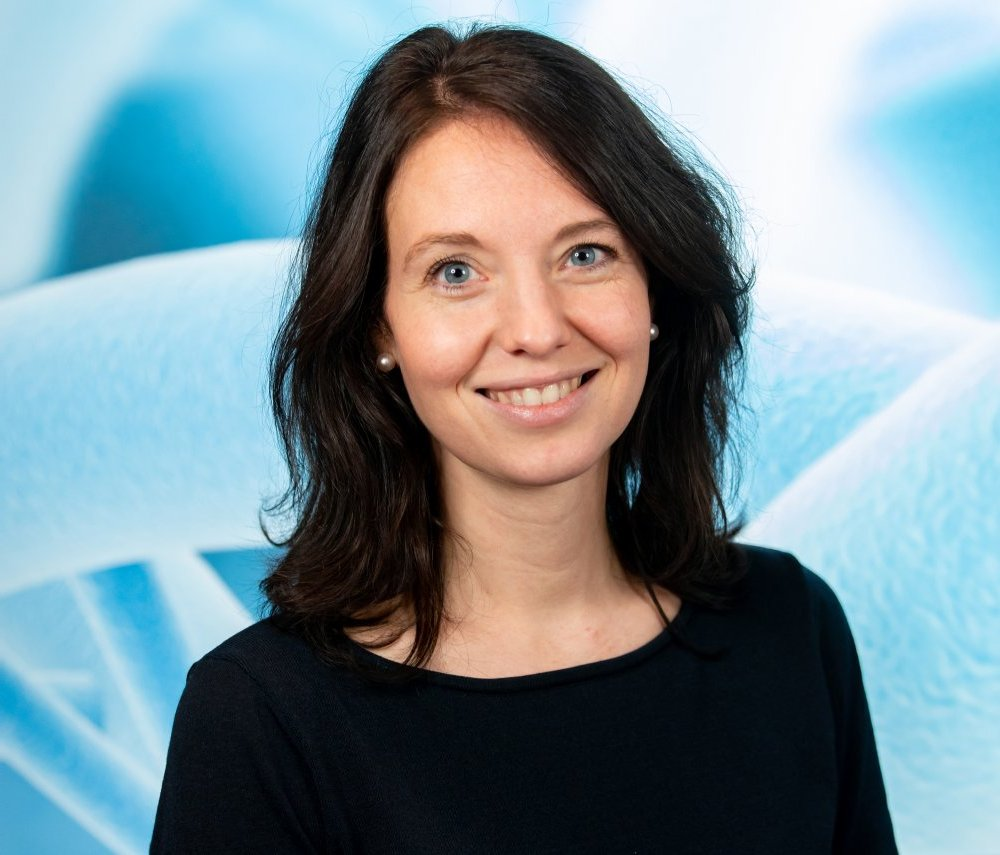
\includegraphics[width=0.2\textwidth]{images/Moerel}
\end{wrapfigure}

\noindent{}A limited number of merit based travel awards, given based on review of summaries by the program committee, are available to presenting students and postdocs who are OCNS members. Women and members of other historically marginalized communities in Science, Technology, Engineering, and Mathematics are particularly encouraged to apply.
Applications for travel grants are to be submitted during the abstract submission process at the annual OCNS conference.

This year's travel awards were competitive, with many more excellent applicants than available funds.
We were pleased to award 19 travel grants to participants from all over the world:

\begin{multicols}{2}
    \begin{itemize}
      \item Flavio Rusch (Brazil)
      \item Cecilia Jarne (Argentina)
      \item Paolo Protachevicz (Brazil)
      \item Fernando Fagundes Ferreira (Brazil)
      \item Pamela Alejandra Illescas Maldonado (Chile)
      \item Lavinia Mitiko Takarabe (Brazil)
      \item Forough Habibollahi Saatlou (Australia)
      \item Fabio Pioggio (Italy)
      \item Richard Gast (USA)
      \item Alexandra Chatzikalymniou (USA)
      \item Ankur Sinha (UK)
      \item Christopher Earl (USA)
      \item Anaelle De Worm (Belgium)
      \item Ferdinand Tixidre (France)
      \item Camille Mazzara (Italy)
      \item Lindsay Stolting (USA)
      \item Elnaz Nemati (Australia)
      \item Dirk Goldschmitt (UK)
      \item Eleonora Bernasconi (UK)
    \end{itemize}
\end{multicols}
\vspace{2ex}
\clearpage
\section*{CNS*2024 Natal: Quotes from a few travel awardees}%
\sectionauthor{\vspace{-4ex}}
%\noindent{}{\color{Blue}\textbf{\large Quotes from a few travel awardees:\\}}

\noindent{}\textbf{Flavio Rusch (Brazil)}
\begin{displayquote}
Attending CNS*2024 was an invaluable experience in my career as a physicist working in computational neuroscience. It provided me the opportunity to present my research to leading figures in the field, engage in discussions, and expand my network of collaborations. I am deeply grateful to OCNS for the travel award, as it made this opportunity possible.
\end{displayquote}

\vspace{2ex}
\noindent{}\textbf{Fabio Poggio (Italy)}
\begin{displayquote}
Receiving the travel award to attend CNS 2024 was a significant opportunity to engage with the latest advances in computational neuroscience and to exchange ideas with leading experts in the field. This experience has significantly enriched my research and professional growth, and I highly recommend it to anyone passionate about computational neuroscience.
\end{displayquote}

\vspace{2ex}
\noindent{}\textbf{Pamela Illescas (Chile)}
\begin{displayquote}
CNS 2024 in Natal was a wonderful experience to learn and share my doctoral thesis on networks with neuron-astrocyte interactions, which allowed
me to receive feedback from other researchers and opportunities for collaboration. This meeting was my first international computational neuroscience conference, and it was possible thanks to the CNS travel award. I am very grateful for this opportunity because it allows me to contribute to computational neuroscience in my country and internationally.
\end{displayquote}

\vspace{2ex}
\noindent{}\textbf{Cecilia Jarne, (Argentina)}
\begin{displayquote}
Attending CNS 2024 was an invaluable experience that allowed me to share our work on Hidden Markov Models (HMMs) software through the tutorial sessions offered at the conference. It also allowed me to present a poster on my ongoing research in predicting brain age, fostering meaningful discussions. I am very grateful for the travel award, which made this enriching experience possible.
\end{displayquote}


